% This LaTeX was auto-generated from MATLAB code.
% To make changes, update the MATLAB code and export to LaTeX again.

\documentclass{article}

\usepackage[utf8]{inputenc}
\usepackage[T1]{fontenc}
\usepackage{lmodern}
\usepackage{graphicx}
\usepackage{color}
\usepackage{hyperref}
\usepackage{amsmath}
\usepackage{amsfonts}
\usepackage{epstopdf}
\usepackage[table]{xcolor}
\usepackage{matlab}
\usepackage[paperheight=845pt,paperwidth=597pt,top=36pt,bottom=36pt,right=36pt,left=36pt,heightrounded]{geometry}

\sloppy
\epstopdfsetup{outdir=./}
\graphicspath{ {./ev_energy_model_realistic_media/} }

\begin{document}

\begin{matlabcode}
clc;
clear;
close all;

% =================================================
\end{matlabcode}


\matlabheading{PART 1: VEHICLE PARAMETERS}

\begin{par}
\begin{flushleft}
=================================================
\end{flushleft}
\end{par}

\begin{matlabcode}
m = 1800;                 % Vehicle mass (kg)
g = 9.81;                 % Gravity (m/s^2)
Crr = 0.01;               % Rolling resistance coefficient
rho = 1.225;              % Air density (kg/m^3)
Cd = 0.29;                % Drag coefficient
A = 2.2;                  % Frontal area (m^2)

delta = 0.08;             % Rotational Mass factor
m_eq = m*(1 + delta);

r_wheel = 0.3;            % Wheel radius (m)

% =================================================
\end{matlabcode}


\matlabheading{PART 2: IMPORT UDDS DRIVE CYCLE}

\begin{par}
\begin{flushleft}
=================================================
\end{flushleft}
\end{par}

\begin{matlabcode}
udds_data = readtable("uddsdc.csv");

t = udds_data.UDDS;       % Time (s)
v_mph = udds_data.Var2;   % Speed (mph)

v = v_mph * 0.44704;      % Convert mph → m/s

dt = mean(diff(t));

a = [diff(v)/dt; 0];      % Acceleration

% Acceleration limits
a_max = 3;
a_min = -4;

a(a>a_max) = a_max;
a(a<a_min) = a_min;

% =================================================
\end{matlabcode}


\matlabheading{PART 3: LONGITUDINAL FORCES}

\begin{par}
\begin{flushleft}
=================================================
\end{flushleft}
\end{par}

\begin{matlabcode}
gear_ratio = 9;

omega_wheel = v / r_wheel;
omega = omega_wheel * gear_ratio;

F_rr   = m * g * Crr;
F_aero = 0.5 * rho * Cd * A .* v.^2;
F_acc  = m_eq .* a;

theta = deg2rad(2);
F_rg = m*g*sin(theta);

F_total = F_rr + F_aero + F_acc + F_rg;

% =================================================
\end{matlabcode}


\matlabheading{PART 4: WHEEL MECHANICAL POWER}

\begin{par}
\begin{flushleft}
=================================================
\end{flushleft}
\end{par}

\begin{matlabcode}
P_wheel = F_total .* v;

eta_tire = 0.95;
P_wheel = P_wheel / eta_tire;

% =================================================
\end{matlabcode}


\matlabheading{PART 5: MOTOR + REGEN LIMITS}

\begin{par}
\begin{flushleft}
=================================================
\end{flushleft}
\end{par}

\begin{matlabcode}
T_motor_max = 250;
T_regen_max = 120;
P_motor_max = 80e3;

v_min_regen = 1.5;

eta_drivetrain = 0.95;

P_mech = zeros(size(P_wheel));

omega_base = P_motor_max / T_motor_max;

for i = 1:length(P_wheel)

    if P_wheel(i) > 0

        if omega(i) <= omega_base
            T_avail = T_motor_max;
        else
            T_avail = P_motor_max / omega(i);
        end

        P_avail = T_avail * omega(i);

        P_mech(i) = min(P_wheel(i), P_avail);

    elseif P_wheel(i) < 0 && v(i) > v_min_regen

        P_regen_limit = T_regen_max * omega(i);

        P_mech(i) = -min(abs(P_wheel(i)), P_regen_limit);

    else

        P_mech(i) = 0;

    end

end

% drivetrain efficiency
P_mech = P_mech / eta_drivetrain;

% =================================================
\end{matlabcode}


\matlabheading{PART 6: DISTANCE \& IDEAL ENERGY}

\begin{par}
\begin{flushleft}
=================================================
\end{flushleft}
\end{par}

\begin{matlabcode}
E_Wh = trapz(t, P_mech) / 3600;

dist_km = trapz(t, v) / 1000;

E_Wh_per_km = E_Wh / dist_km;

% =================================================
\end{matlabcode}


\matlabheading{PART 7: MOTOR + INVERTER EFFICIENCY}

\begin{par}
\begin{flushleft}
=================================================
\end{flushleft}
\end{par}

\begin{matlabcode}
omega_max = max(omega) + eps;

drive_eff = ones(size(P_mech));
regen_eff = ones(size(P_mech));

for i = 1:length(P_mech)

    if P_mech(i) > 0

        T_req = P_mech(i) / max(omega(i),eps);

        Tn = abs(T_req) / T_motor_max;

        on = omega(i) / omega_max;

        drive_eff(i) = 0.90 ...
            - 0.15*(1-on)^2 ...
            - 0.20*(Tn-0.6)^2;

        drive_eff(i) = min(max(drive_eff(i),0.75),0.92);

    elseif P_mech(i) < 0

        T_req = abs(P_mech(i)) / max(omega(i),eps);

        Tn = T_req / T_regen_max;

        on = omega(i) / omega_max;

        regen_eff(i) = 0.75 ...
            - 0.20*(1-on)^2 ...
            - 0.30*(Tn-0.5)^2;

        regen_eff(i) = min(max(regen_eff(i),0.55),0.80);

    end

end

% =================================================
\end{matlabcode}


\matlabheading{PART 8: BATTERY POWER FLOW}

\begin{par}
\begin{flushleft}
=================================================
\end{flushleft}
\end{par}

\begin{matlabcode}
P_batt_disch_max = 90e3;
P_batt_char_max  = 40e3;

P_accessory = 900;

Batt_capacity = 50; % kWh

P_drive = zeros(size(P_mech));
P_regen = zeros(size(P_mech));

for i = 1:length(P_mech)

    if P_mech(i) > 0

        P_drive(i) = P_mech(i) / drive_eff(i);

        P_drive(i) = min(P_drive(i), P_batt_disch_max);

    elseif P_mech(i) < 0

        P_regen(i) = abs(P_mech(i)) * regen_eff(i);

        P_regen(i) = min(P_regen(i), P_batt_char_max);

    end

end

P_batt = P_drive - P_regen + P_accessory;

% =================================================
\end{matlabcode}


\matlabheading{PART 9: SOC MODEL}

\begin{par}
\begin{flushleft}
=================================================
\end{flushleft}
\end{par}

\begin{matlabcode}
SOC = zeros(size(t));

SOC(1) = 0.80;

for i = 2:length(t)

    E_step_Wh = P_batt(i) * dt / 3600;

    SOC(i) = SOC(i-1) - E_step_Wh/(Batt_capacity*1000);

end

% =================================================
\end{matlabcode}


\matlabheading{PART 10: PLOTS}

\begin{par}
\begin{flushleft}
=================================================
\end{flushleft}
\end{par}

\begin{matlabcode}
figure('Name','EV UDDS Simulation');

subplot(3,1,1)
plot(t,v*3.6,'r','LineWidth',1.5)
xlabel('Time (s)')
ylabel('Speed (km/h)')
title('UDDS Drive Cycle')
grid on

subplot(3,1,2)
plot(t,P_drive/1000,'b'); hold on
plot(t,-P_regen/1000,'g')
xlabel('Time (s)')
ylabel('Power (kW)')
legend('Drive','Regen')
title('Battery Power Flow')
grid on

subplot(3,1,3)
plot(t,SOC*100,'k','LineWidth',1.5)
xlabel('Time (s)')
ylabel('SOC (%)')
title('Battery State of Charge')
grid on
\end{matlabcode}
\begin{center}
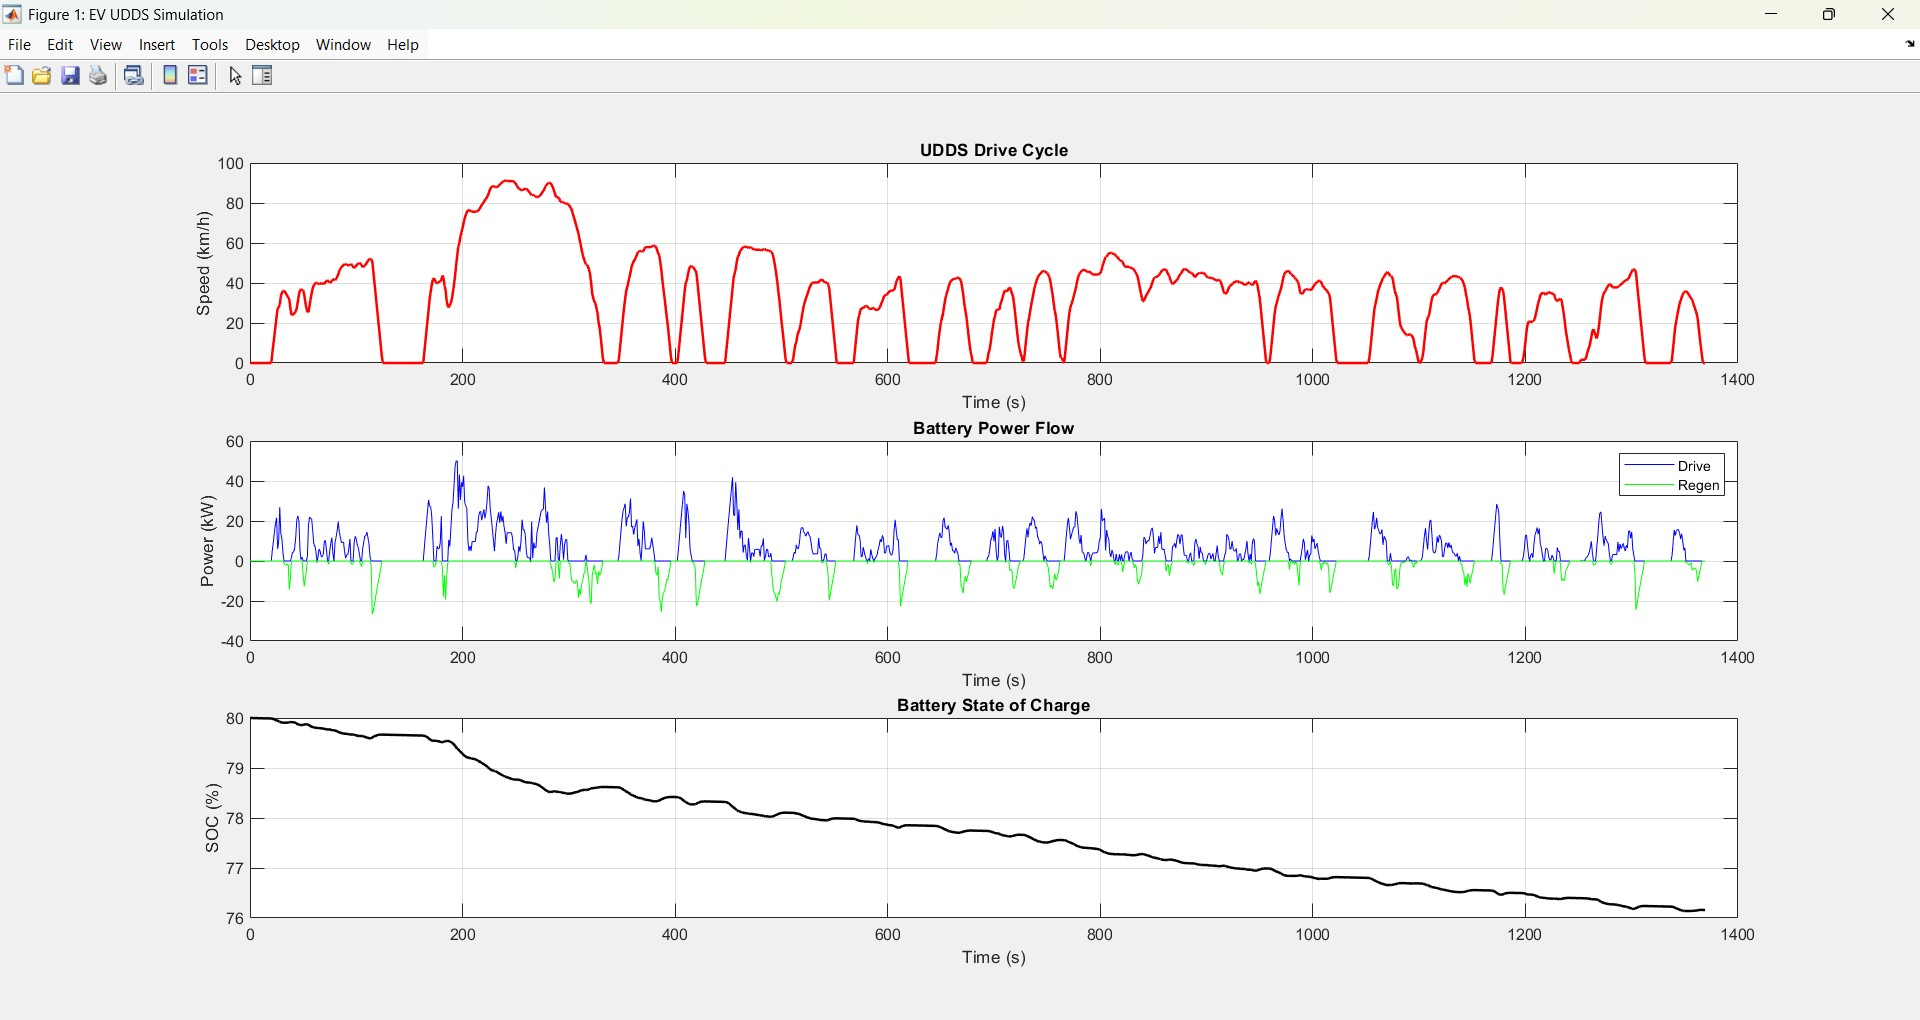
\includegraphics[width=\maxwidth{56.196688409433015em}]{figure_0.jpeg}
\end{center}
\begin{matlabcode}

% =================================================
\end{matlabcode}


\matlabheading{PART 11: FINAL RESULTS}

\begin{par}
\begin{flushleft}
=================================================
\end{flushleft}
\end{par}

\begin{matlabcode}
E_drive_Wh = trapz(t,P_drive)/3600;

E_regen_Wh = trapz(t,P_regen)/3600;

E_batt_net = E_drive_Wh - E_regen_Wh;

E_brake_mech = trapz(t,abs(min(P_mech,0)))/3600;

regen_percentage = (E_regen_Wh/E_brake_mech)*100;

P_drive_max = max(P_drive)/1000;

P_regen_max = max(P_regen)/1000;

P_wheel_max = max(P_mech)/1000;

SOC_initial = SOC(1)*100;

SOC_final = SOC(end)*100;

SOC_delta = SOC_initial - SOC_final;

avg_speed_kmh = mean(v)*3.6;

% =================================================
\end{matlabcode}


\matlabheading{PRINT RESULTS}

\begin{par}
\begin{flushleft}
=================================================
\end{flushleft}
\end{par}

\begin{matlabcode}
fprintf('\nVEHICLE & DRIVE CYCLE\n\n');
\end{matlabcode}
\begin{matlaboutput}
VEHICLE & DRIVE CYCLE
\end{matlaboutput}
\begin{matlabcode}

fprintf('Vehicle Mass\n: %.0f kg\n\n',m);
\end{matlabcode}
\begin{matlaboutput}
Vehicle Mass
: 1800 kg
\end{matlaboutput}
\begin{matlabcode}

fprintf('Total Distance Travelled\n: %.3f km\n\n',dist_km);
\end{matlabcode}
\begin{matlaboutput}
Total Distance Travelled
: 11.990 km
\end{matlaboutput}
\begin{matlabcode}

fprintf('Average Speed\n: %.2f km/h\n\n',avg_speed_kmh);
\end{matlabcode}
\begin{matlaboutput}
Average Speed
: 31.51 km/h
\end{matlaboutput}
\begin{matlabcode}

fprintf('Drive Cycle Duration\n: %.0f s\n\n',t(end));
\end{matlabcode}
\begin{matlaboutput}
Drive Cycle Duration
: 1369 s
\end{matlaboutput}
\begin{matlabcode}


fprintf('ENERGY CONSUMPTION\n\n');
\end{matlabcode}
\begin{matlaboutput}
ENERGY CONSUMPTION
\end{matlaboutput}
\begin{matlabcode}

fprintf('Wheel Mechanical Energy\n: %.2f Wh\n\n',E_Wh);
\end{matlabcode}
\begin{matlaboutput}
Wheel Mechanical Energy
: 3086.55 Wh
\end{matlaboutput}
\begin{matlabcode}

fprintf('Battery Energy Drawn\n: %.2f Wh\n\n',E_drive_Wh);
\end{matlabcode}
\begin{matlaboutput}
Battery Energy Drawn
: 4413.01 Wh
\end{matlaboutput}
\begin{matlabcode}

fprintf('Battery Energy Regenerated\n: %.2f Wh\n\n',E_regen_Wh);
\end{matlabcode}
\begin{matlaboutput}
Battery Energy Regenerated
: 366.46 Wh
\end{matlaboutput}
\begin{matlabcode}

fprintf('Net Battery Energy Used\n: %.2f Wh\n\n',E_batt_net);
\end{matlabcode}
\begin{matlaboutput}
Net Battery Energy Used
: 4046.55 Wh
\end{matlaboutput}
\begin{matlabcode}

fprintf('Specific Energy Consumption\n: %.2f Wh/km\n\n',E_batt_net/dist_km);
\end{matlabcode}
\begin{matlaboutput}
Specific Energy Consumption
: 337.49 Wh/km
\end{matlaboutput}
\begin{matlabcode}


fprintf('POWER PERFORMANCE\n\n');
\end{matlabcode}
\begin{matlaboutput}
POWER PERFORMANCE
\end{matlaboutput}
\begin{matlabcode}

fprintf('Maximum Wheel Power\n: %.2f kW\n\n',P_wheel_max);
\end{matlabcode}
\begin{matlaboutput}
Maximum Wheel Power
: 53.55 kW
\end{matlaboutput}
\begin{matlabcode}

fprintf('Maximum Battery Drive Power\n: %.2f kW\n\n',P_drive_max);
\end{matlabcode}
\begin{matlaboutput}
Maximum Battery Drive Power
: 61.42 kW
\end{matlaboutput}
\begin{matlabcode}

fprintf('Maximum Regen Power\n: %.2f kW\n\n',P_regen_max);
\end{matlabcode}
\begin{matlaboutput}
Maximum Regen Power
: 20.32 kW
\end{matlaboutput}
\begin{matlabcode}


fprintf('REGENERATIVE BRAKING\n\n');
\end{matlabcode}
\begin{matlaboutput}
REGENERATIVE BRAKING
\end{matlaboutput}
\begin{matlabcode}

fprintf('Mechanical Braking Energy\n: %.2f Wh\n\n',E_brake_mech);
\end{matlabcode}
\begin{matlaboutput}
Mechanical Braking Energy
: 561.29 Wh
\end{matlaboutput}
\begin{matlabcode}

fprintf('Regen Energy Recovery\n: %.2f %%\n\n',regen_percentage);
\end{matlabcode}
\begin{matlaboutput}
Regen Energy Recovery
: 65.29 %
\end{matlaboutput}
\begin{matlabcode}


fprintf('BATTERY STATE OF CHARGE\n\n');
\end{matlabcode}
\begin{matlaboutput}
BATTERY STATE OF CHARGE
\end{matlaboutput}
\begin{matlabcode}

fprintf('Initial SOC\n: %.2f %%\n\n',SOC_initial);
\end{matlabcode}
\begin{matlaboutput}
Initial SOC
: 80.00 %
\end{matlaboutput}
\begin{matlabcode}

fprintf('Final SOC\n: %.2f %%\n\n',SOC_final);
\end{matlabcode}
\begin{matlaboutput}
Final SOC
: 71.22 %
\end{matlaboutput}
\begin{matlabcode}

fprintf('Net SOC Change\n: %.3f %%\n\n',SOC_delta);
\end{matlabcode}
\begin{matlaboutput}
Net SOC Change
: 8.778 %
\end{matlaboutput}
\begin{matlabcode}


% =================================================
\end{matlabcode}


\matlabheading{MOTOR TORQUE SPEED CHARACTERISTIC}

\begin{par}
\begin{flushleft}
=================================================
\end{flushleft}
\end{par}

\begin{matlabcode}
omega_range = linspace(0, max(omega)*1.2, 500);

T_motor = zeros(size(omega_range));

for i = 1:length(omega_range)

    if omega_range(i) <= omega_base
        T_motor(i) = T_motor_max;
    else
        T_motor(i) = P_motor_max / omega_range(i);
    end

end

figure

plot(omega_range, T_motor,'LineWidth',2);

xlabel('Motor Speed (rad/s)');
ylabel('Torque (Nm)');
title('EV Motor Torque-Speed Curve');

grid on;
\end{matlabcode}
\begin{center}
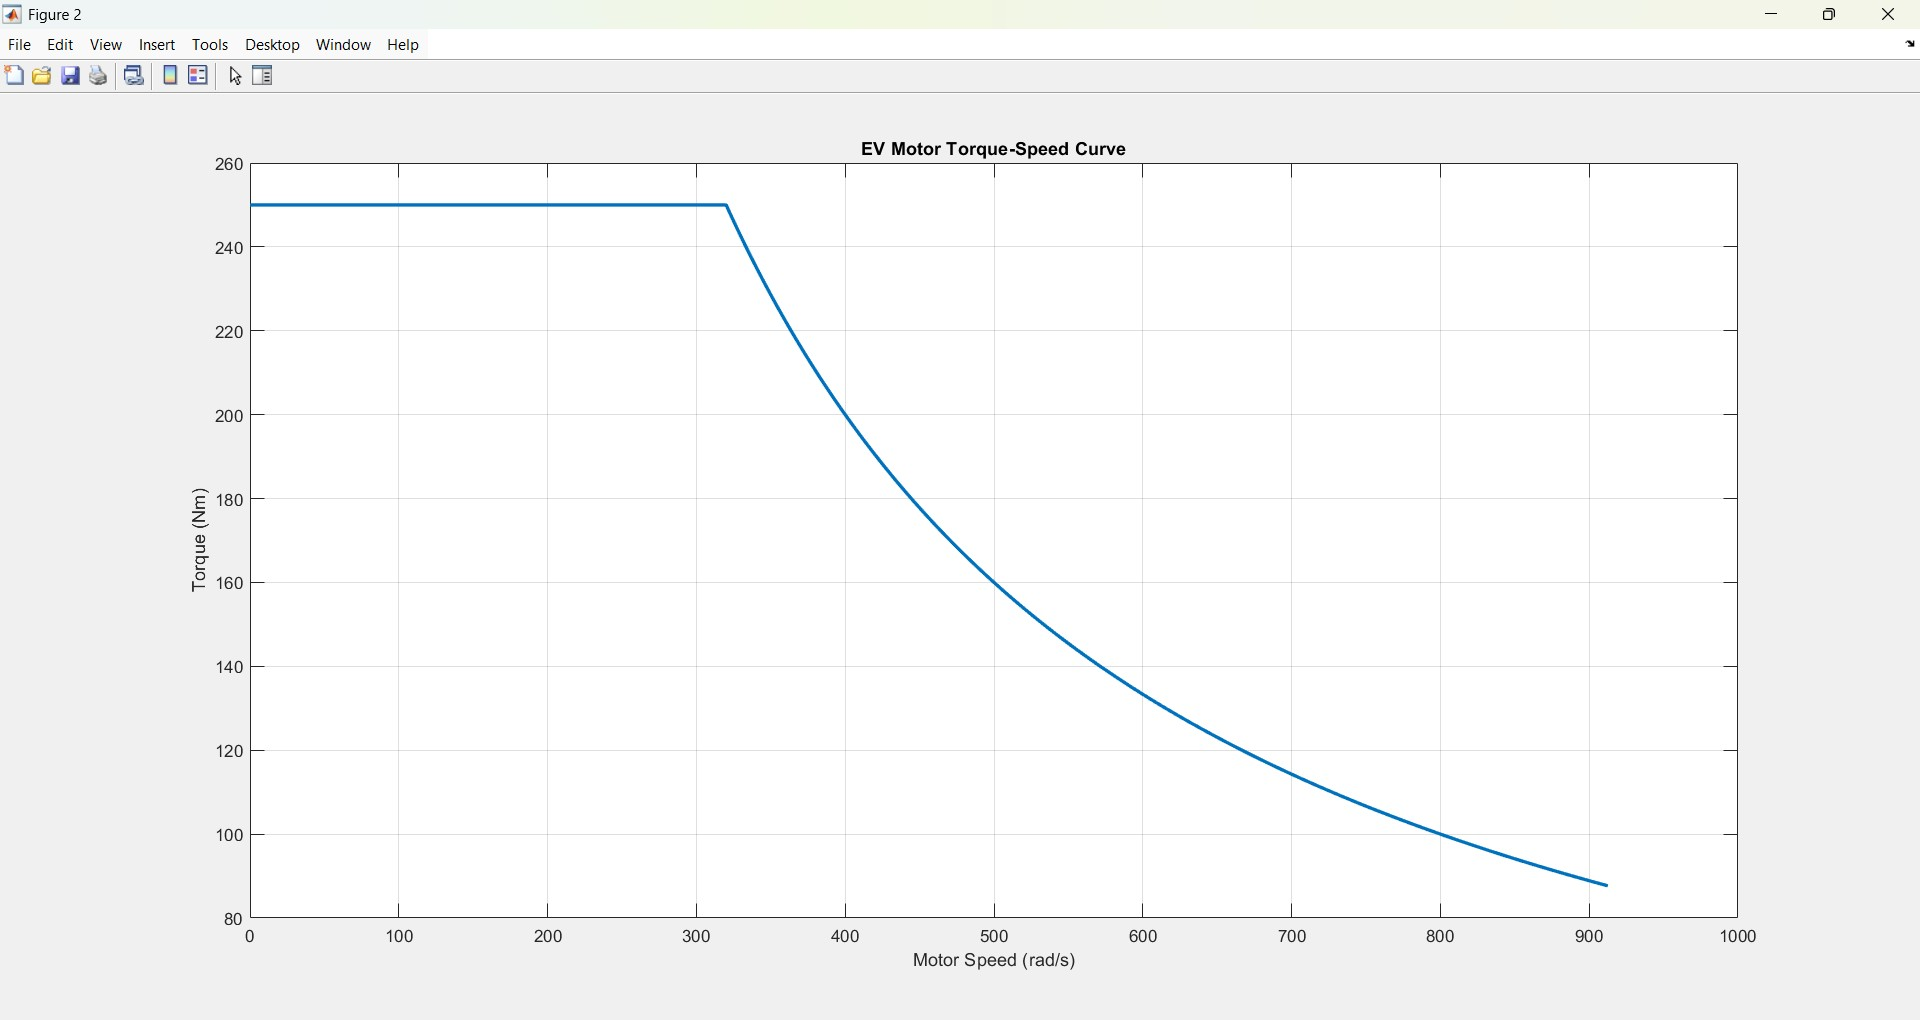
\includegraphics[width=\maxwidth{56.196688409433015em}]{figure_1.jpeg}
\end{center}
\begin{matlabcode}

% =================================================
\end{matlabcode}


\matlabheading{MOTOR EFFICIENCY MAP}

\begin{par}
\begin{flushleft}
=================================================
\end{flushleft}
\end{par}

\begin{matlabcode}
speed_norm = omega/omega_max;

torque = P_mech ./ max(omega,eps);

torque_norm = abs(torque)/T_motor_max;

figure

scatter(speed_norm, torque_norm, 15, drive_eff,'filled')

colorbar

xlabel('Normalized Speed');
ylabel('Normalized Torque');

title('Motor Efficiency Map');

grid on;
\end{matlabcode}
\begin{center}
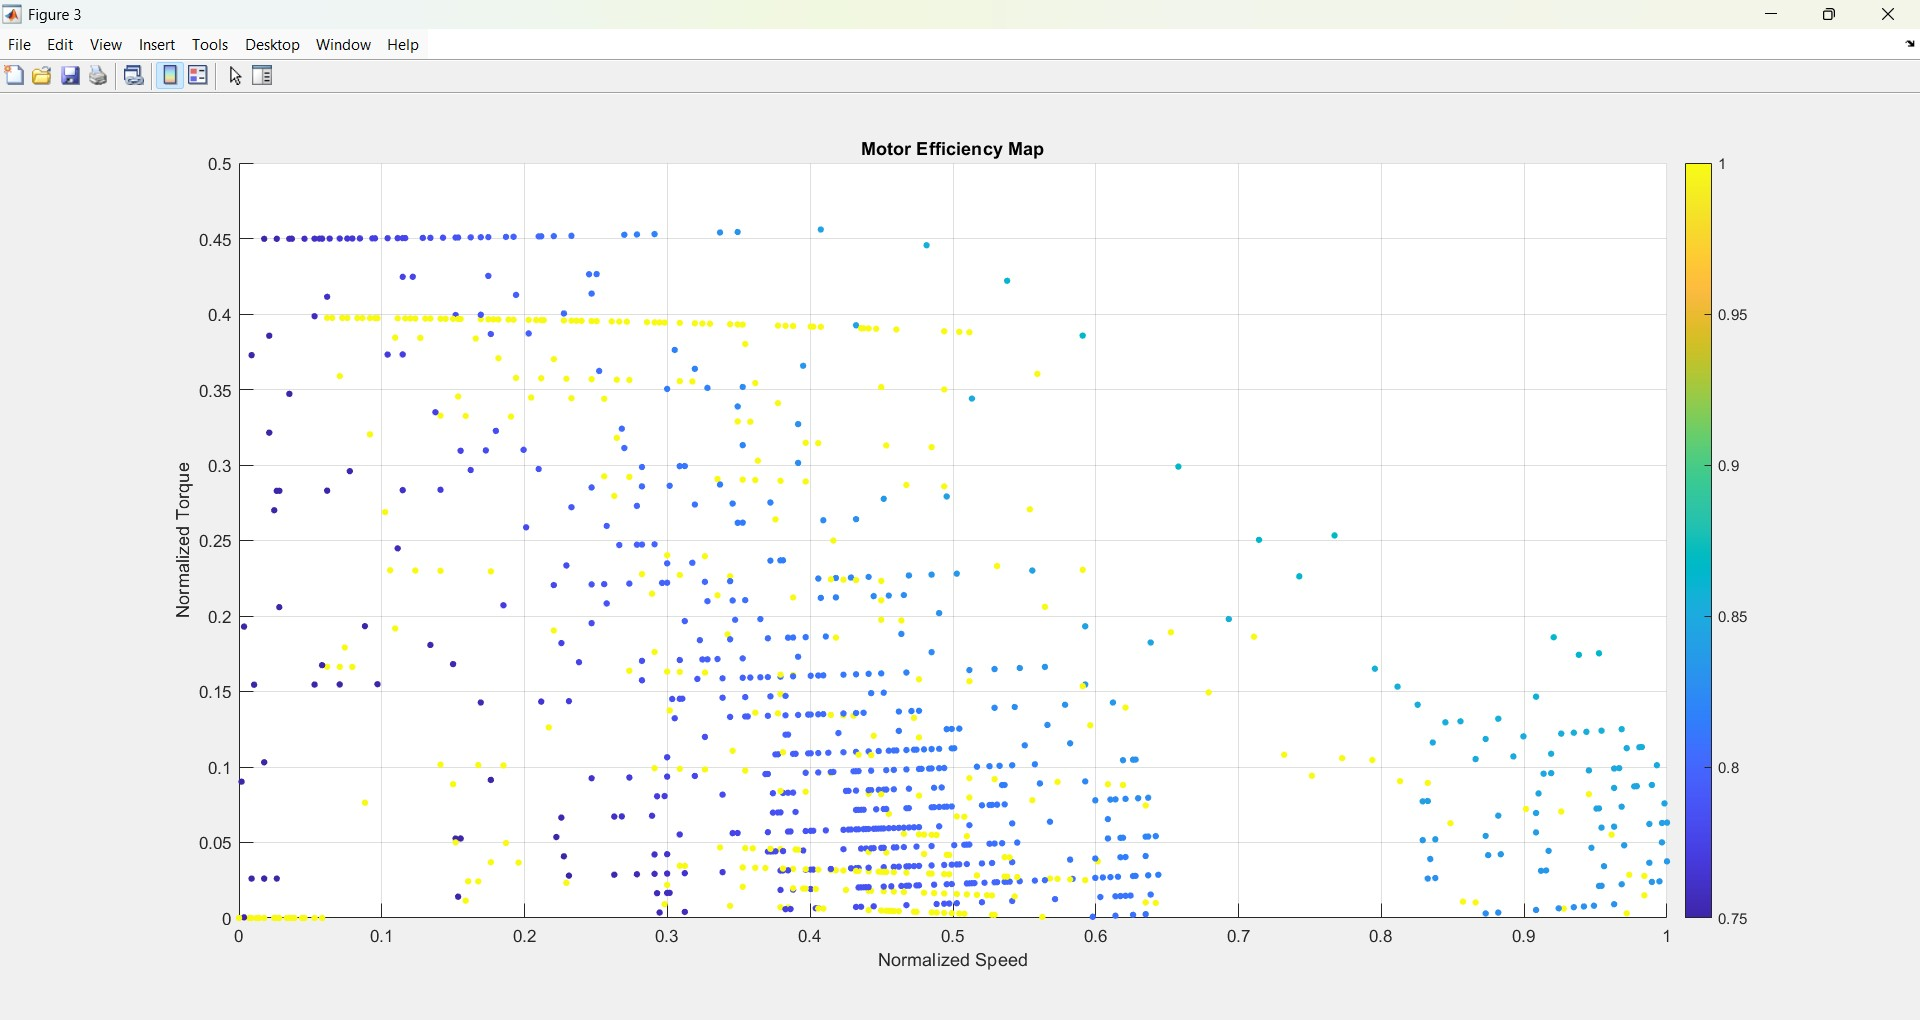
\includegraphics[width=\maxwidth{56.196688409433015em}]{figure_2.jpeg}
\end{center}
\begin{matlabcode}

% =================================================
\end{matlabcode}


\matlabheading{ENERGY FLOW ANALYSIS}

\begin{par}
\begin{flushleft}
=================================================
\end{flushleft}
\end{par}

\begin{matlabcode}
E_accessory = trapz(t, ones(size(t))*P_accessory)/3600;

fprintf('\nENERGY FLOW ANALYSIS\n\n');
\end{matlabcode}
\begin{matlaboutput}
ENERGY FLOW ANALYSIS
\end{matlaboutput}
\begin{matlabcode}

fprintf('Drive Energy From Battery : %.2f Wh\n',E_drive_Wh);
\end{matlabcode}
\begin{matlaboutput}
Drive Energy From Battery : 4413.01 Wh
\end{matlaboutput}
\begin{matlabcode}

fprintf('Recovered Regen Energy    : %.2f Wh\n',E_regen_Wh);
\end{matlabcode}
\begin{matlaboutput}
Recovered Regen Energy    : 366.46 Wh
\end{matlaboutput}
\begin{matlabcode}

fprintf('Accessory Consumption     : %.2f Wh\n',E_accessory);
\end{matlabcode}
\begin{matlaboutput}
Accessory Consumption     : 342.25 Wh
\end{matlaboutput}
\begin{matlabcode}

fprintf('Net Battery Consumption   : %.2f Wh\n',E_batt_net);
\end{matlabcode}
\begin{matlaboutput}
Net Battery Consumption   : 4046.55 Wh
\end{matlaboutput}
\begin{matlabcode}



% =================================================
\end{matlabcode}


\matlabheading{RANGE ESTIMATION}

\begin{par}
\begin{flushleft}
=================================================
\end{flushleft}
\end{par}

\begin{matlabcode}
usable_SOC = 0.8 - 0.2;   % 80% to 20%

usable_energy = Batt_capacity * usable_SOC * 1000; % Wh

range_est = usable_energy / (E_batt_net/dist_km);

fprintf('\nESTIMATED EV RANGE\n\n');
\end{matlabcode}
\begin{matlaboutput}
ESTIMATED EV RANGE
\end{matlaboutput}
\begin{matlabcode}

fprintf('Estimated Range (UDDS Based) : %.1f km\n',range_est);
\end{matlabcode}
\begin{matlaboutput}
Estimated Range (UDDS Based) : 88.9 km
\end{matlaboutput}

\end{document}
